\nTitle{Conception}

%%%%%%%%%%%%%%%%%%%%%%%%%%%%%%%%%%%%%%%%%%%%%%%%%%%%%%%%%%%%
\section{Rappel du contexte}
% Martin


%%%%%%%%%%%%%%%%%%%%%%%%%%%%%%%%%%%%%%%%%%%%%%%%%%%%%%%%%%%%
\section{Choix d'une solution}
\subsection{Présentation des alternatives}

\subsubsection{Points commun des trois solutions}
% Yoann
À l'ouverture d'un fichier, son contenu est copié dans un fichier temporaire --- éventuellement en le structurant de manière adaptée à l'éditeur. Le fichier est indexé de manière à pouvoir accéder aux lignes directement.

Un tampon de taille limitée est créé en mémoire centrale. Lorsque l'utilisateur demande à accéder à des lignes qui n'y sont pas encore chargées, les lignes les plus anciennement accédées sont remplacées par celles qui viennent d'être demandées.

Le tampon est modifié directement au fur et à mesure de la frappe de l'utilisateur, et la ligne modifiée est transférée dans le fichier temporaire dès que l'utilisateur passe à une nouvelle ligne ou demande une sauvegarde du fichier. Le fichier source, quant à lui, est mis à jour sur demande de l'utilisateur (sauvegarde du fichier).

\subsubsection{Solution 1 : structure consécutive}
% Paul

\subsubsection{Solution 2 : structure mixte}
% Martin

\subsubsection{Solution 3 : structure chaînée}
% Yoann
Toutes les structures de données sont chaînées.

Le ficher temporaire est chaîné grâce à des adresses virtuelles, comme présentées ci-dessous.

\begin{figure}[H]
	\centering
	\caption{Structure d'une adresse virtuelle}
	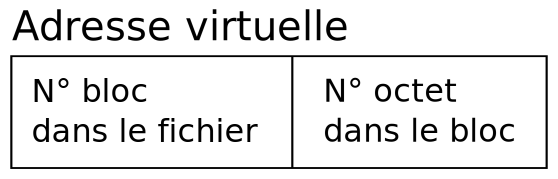
\includegraphics[width=0.5\textwidth]{structure_chainee_temp_adresse_virtuelle}
\end{figure}

Ainsi chaque ligne (y compris la \og ligne 0 \fg virtuelle) fait référence à son successeur et son prédécesseur. On stocke également la longueur de l'information (\og longueur utile \fg) et le nombre d'octets disponibles dans l'enregistrement (\og longueur max \fg, supérieure ou égale à la longueur utile).

\begin{figure}[H]
	\centering
	\caption{Structure du fichier temporaire de la solution 3}
	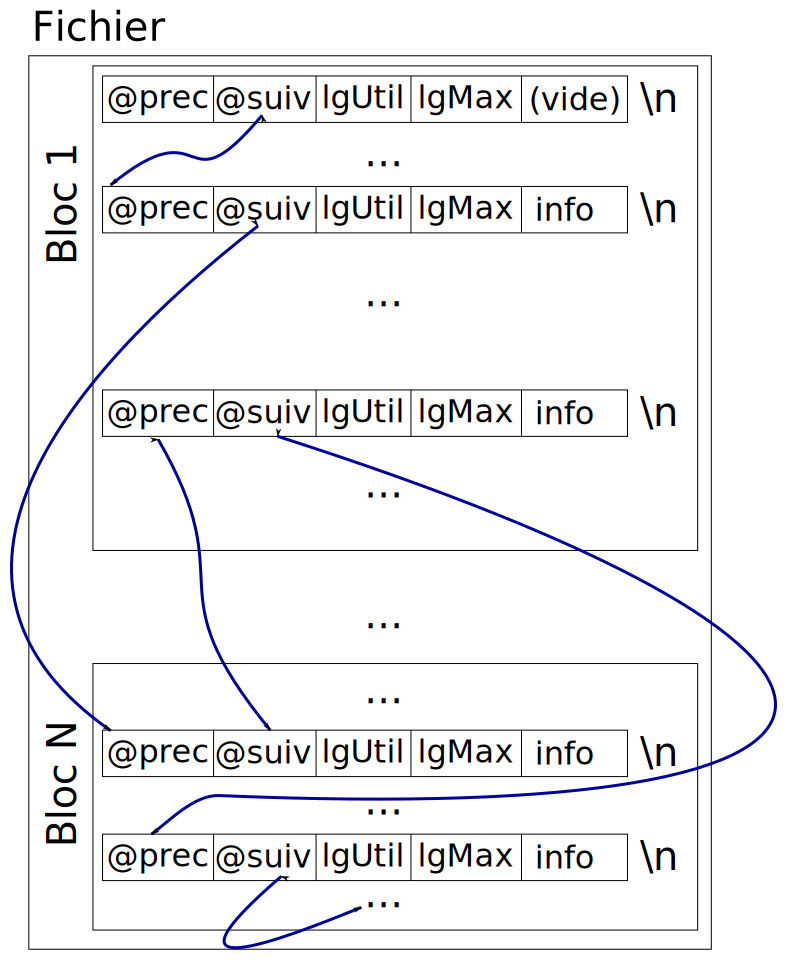
\includegraphics[width=0.6\textwidth]{structure_chainee_temp}
\end{figure}

L'accès direct (lorsque l'utilisateur demande d'accéder à la ligne $l$, par exemple) est possible toutes les $L$ lignes ($L$ à définir) grâce à la table de \textsl{mapping}, qui donne pour chaque bloc la dernière ligne stockée dans celui-ci. Cette table est bien sûr complétée et mise à jour au fur et à mesure de l'édition du fichier (suppressions, ajouts, \ldots). Pour accéder à une ligne non indexée, il suffit d'accéder à une ligne proche et indexée, et de suivre le chaînage (complexité bornée).

Cette table contient bien sûr d'autres informations, comme le montre la représentation suivante.

\newcommand{\TableSolTroisHLine}{\cline{1-5} \cdashline{6-6} \cline{7-7}}
\begin{figure}[H]
	\centering
	\caption{Structure de la table de \textsl{mapping} de la solution 3}
	\vspace{3mm}
	\begin{tabular}{|c|c|c|c|c|c|c|}
		N\textdegree{} ligne & N\textdegree{} bloc & Octet & Chargé & Date dernier accès & (Autres infos) & Adresse MC \\
		\TableSolTroisHLine
		10 & 1 & 156 & Non & 1289135888657534079 & \ldots & \texttt{0x000000}\\
		\TableSolTroisHLine
		\multicolumn{7}{:c:}{} \\
		\multicolumn{7}{:c:}{\ldots} \\
		\multicolumn{7}{:c:}{} \\
		\TableSolTroisHLine
		119 & N & 451 & Oui & 1289135888658945079 & \ldots & \texttt{0x4006d4}\\
		\TableSolTroisHLine
	\end{tabular}
\end{figure}




\subsection{Comparaison des alternatives}
% En commun
% « Mécanisme de justification » : un tableau avec des « + » et des « - » ?
\begin{table}[H]
	\centering
	\caption{Table comparative des avantages et inconvénients de chaque solution}
	\begin{tabular}{l|c|c|c}
		Critère & Solution 1 & Solution 2 & Solution 3 \\
		\hline
		??? & & & \\
		??? & & & \\
		??? & & & \\
		??? & & & \\
		??? & & &
	\end{tabular}
\end{table}



%%%%%%%%%%%%%%%%%%%%%%%%%%%%%%%%%%%%%%%%%%%%%%%%%%%%%%%%%%%%
\section{Détail de la solution choisie}

\subsection{...}

\subsection{...}

\subsection{...}

\subsection{...}

\subsection{Proposition d'architecture}
% Découpage modulaire et hiérarchique


%%%%%%%%%%%%%%%%%%%%%%%%%%%%%%%%%%%%%%%%%%%%%%%%%%%%%%%%%%%%
\section{Bilan}
% Bilan de la solution choisie par rapport aux exigeances + réflexions personnelles
